\section{Chapter 2 Questions}
\subsection{Short Answer}
\begin{enumerate}
    \item At which layer of the OSI model does a proxy exist?\\Layer 7, application.
    \item If a device is using node MAC (media access control) address to funnel traffic, what layer of OSI model is this device working on?\\Layer 2 (data link layer).
    %\item Which OS holds 90 percent of the desktop market and is one of out largest attack surfaces?\\Windows.
    \item Which port uses SSL to secure web traffic?\\443.
    \item What kind of domain resides on a single switch-port?\\Collision domain.
    \item Which network topology uses a token-based access methodology?\\Ring
    \item Hubs operate at what layer of the OSI model?\\Layer 1
    \item What is the proper sequence of the TCP three-way-handshake?\\SYN, SYN-ACK, ACK
    \item Which of these protocols is a connection-oriented protocol?\\TCP
    \item A scan of a network client show that port 23 is open; What protocol is this aligned with?\\Telnet
    \item What port range is an obscure third-party application most likely to use?\\49152 to 65535
    \item Which category of 'firewall filters' is based on packet header data only?\\Packet filter
    \item An administrator has just been notified of irregular network activity; what appliance functions in this manner?\\IDS (Intrusion detection system)
    \item Which topology has built-in redundancy because of its many client connections?\\Mesh
    \item When scanning a network via a hardline connection to a wired-switch NIC, in promiscuous mode, what would be the extent of network traffic you would expect to see?\\All nodes attached to same port.
    \item What device acts as an intermediary between an internal client and a web resource?\\Proxy
    \item Which technology allows the use of a single public address to support many internal clients while also preventing exposure of internal IP addresses to the outside world?\\NAT (Network Address Translation)
    \item What network appliance senses irregularities and plays an active role in stopping that irregular activity from continuing?\\IPS (Intrusion prevention system)
    \item Matthew has selected the option in IDS to notify via email if it senses any network irregularities. Checking the logs, there are incidences but he did not receive any emails. What protocol needs to be enabled on the IDS?\\SMTP.
    \item Choosing a protective network appliance, you want a device that will inspect packets at the most granular level possible, while providing improved traffic efficiency. What appliance would satisfy these requirements?\\Proxy firewall
    \item What is the difference between a traditional firewall and an IPS?\\IPS can dissect packet.
    \item Which of the following options shows the well-known ports?\\
    \item Of the following methods, which one acts as a middleman between an external network and the private network by initiating and establishing the connection?
    \item What are two common ports used to connect to a web server?\\443 and 80
    \item Which two protocols are connectionless?\\IP and UDP
    \item At which layer of the OSI model does FTP reside?
    \item What port is used by DNS?\\53
    \item What would you call an IP address bonding with a port number?
    \item Which of the following allows networks to be sub netted into various sizes in IP4 system as IP6 will take years to be fully implemented?
    \item At what layer does ICMP (internet control message protocol) operate?
    \item What is wrong with the following diagram?
    \begin{figure}[H]
        \centering
        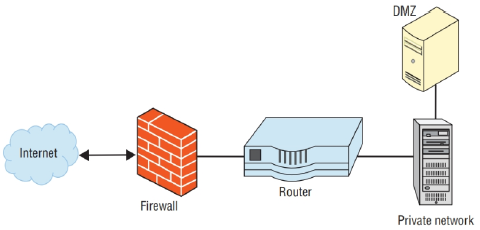
\includegraphics[width=\linewidth]{fig1.png}
    \end{figure}
    The DMZ should be associated with the Internet. The DMZ should reside off the firewall and not directly off from the private network.
    \item What type of network topology is being shown in the following diagram?
    \begin{figure}[H]
        \centering
        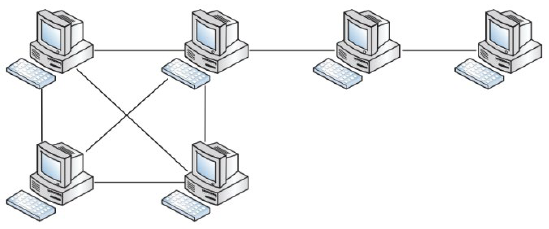
\includegraphics[width=\linewidth]{fig2.png}
    \end{figure}
    \item Which header field is used to reassemble fragmented IP packets?
    \item What for a MAC address used?
\end{enumerate}

\subsection{Long Answer}
\begin{itemize}
    \item Describe types of network. What is importance of Mesh network / hybrid network.\\
    Types of networks vary based on their level of connectivity and redundancy, Bus networks have one connection that every nodes use, the design is simple but hard to troubleshoot if an issue comes up.
    Ring networks are similar to bus networks but provide more redundancy by layering rings.
    Star networks are popular for the ease of setup and troubleshooting, by connecting every node to a central device that ties the network together.
    Mesh and hybrid networks attach groups of nodes to each other, have a high level of redundancy and resistance to outages.
    These are important because our current networks are built and improved off of past networks, creating more complicated structures as networks are expanded, mesh and hybrid networks better support this.
    \item What is ports in computer networking. Write on different categories of ports and their functionalities.\\
    Ports identify types of traffic associated with a protocol or application.
    If you need to connect to the internet, port 80 or 443 will be used depending on if you are connecting via HTTP or HTTPS.
    In our lab we disabled connections on port 80, meaning the client could not connect to a web server via unsecured HTTP, but could connect to a HTTPS webpage.
    Well known ports are between 0 and 1023, registered ports are between 1024 and 49151, dynamic ports are from 49152 to 65535.
    \item Describe on IP address assignment system.\\
    When connecting to a network for the first time DHCP will assign a ip address that connects the MAC address of the device to a single IP on the network.
    This allows connections to be made by using the assigned IP address.
    You can view the IP address via \verb|ipconfig| command in Windows.
    The commaind \verb|ipconfig /release| will free the IP address from you machine and allow it for use on a different machine.
    \verb|ipcocfig /renew| will request a new IP address for the host from DHCP.
    \verb|ipconfig, ipconfig \all, ipconfig \release, ipconfig \renew|
    \item What firewall does. Write on types of firewalls\\
    Firewalls are used to block unwanted or malicious connections by analyzing the packets header information, state of connections or the packet payload for any abnormalities.
    Packet filtering firewalls drop packets by filtering the source and destination addresses, ports, and protocols.
    Stateful firewalls determine if traffic is legitimate based on the state of connection from which the traffic originated.
    Deep packet inspection firewalls look into the payload of the packet for any malware or attack before the packet reaches its destination.
    \item Explain what type of information a packet (computer networking technology) contain.\\
    Packets are small chunks of data passed over networks and have defined sections of information to ensure that the packet will get to its location.
\end{itemize}